
\documentclass{beamer}
\setbeamertemplate{navigation symbols}{}


\usetheme{Warsaw}
\usepackage{ngerman}
\beamersetuncovermixins{\opaqueness<1>{25}}{\opaqueness<2->{15}}

\AtBeginSection[]
{
   \begin{frame}
       \frametitle{Inhalt}
       \tableofcontents[currentsection]
   \end{frame}
}

\begin{document}
\title{BlueHotel}
\author{Alexander Duml, Stefan M\"uller, Thomas Perl \& Martin Wieser}
\date{\today}

\begin{frame}
\titlepage
\end{frame}

\begin{frame}
\frametitle{Inhalt}\tableofcontents
\end{frame}



\section{Team}

\begin{frame}
\frametitle{Mitglieder}
\begin{itemize}
\item Alexander Duml (Entwicklungsteam)
\item Stefan M\"uller (Scrummaster)
\item Thomas Perl (Entwicklungsteam)
\item Martin Wieser (Product Owner)
\end{itemize}
\end{frame}

\section{Prozess}

\begin{frame}
\frametitle{Geplanter Verlauf (1/2)}
\begin{itemize}
\item Rollen bei Dokumentation und jeder ist Entwickler (weitere Rollen vernachl\"assigen)
\item Sprint: Dauer 1 Woche
\end{itemize}
\begin{itemize}
\item Sprint Planning 1 \& 2 (zusammenlegen): am Beginn jeder Woche durchgef\"uhrt
\item Sprint Review \& Retrospective (zusammenlegen): am Ende jeder Woche
\item DailyScrum: nicht durchgef\"uhrt
\end{itemize}
\end{frame}

\begin{frame}
\frametitle{Geplanter Verlauf (2/2)}
\begin{itemize}
\item Product Backlog: in LaTeX (Product Owner)
\item Sprint Backlog, BugListe \& Burndown-Charts: in Excel (Scrum Master)
\item Repository: GitHub
\item Tests: ???
\end{itemize}
\end{frame}

\begin{frame}
\frametitle{Probleme}
\begin{itemize}
\item Tests bei erstem Sprint nicht definiert
\item Viele verschiedene Technologien f\"ur Management
\item Schwierigkeiten bei Terminvereinbarung
\end{itemize}
\end{frame}

\begin{frame}
\frametitle{Tats\"achlicher Verlauf}
\begin{itemize}
\item Rollen bei Dokumentation und jeder ist Entwickler (weitere Rollen vernachl\"assigen)
\item Sprint: Dauer 1 Woche
\end{itemize}
\begin{itemize}
\item Sprint Planning 1 \& 2, Sprint Review \& Retrospective (zusammenlegen): am Ende jeder Woche durchgef\"uhrt
\item DailyScrum: nicht durchgef\"uhrt
\end{itemize}
\begin{itemize}
\item Product Backlog: GitHuB-Wiki
\item Sprint Backlog \& BugListe: GitHub (Issues)
\item Tests: Funktionale Tests + JUnit-Tests
\end{itemize}
\end{frame}

\section{Projekt}

\begin{frame}
\frametitle{Erledigt (1/2 )}
\begin{itemize}
\item  Sprint 1:
\begin{itemize}
\item  Reservierung vornehmen
\item  Kunde anlegen
\item  Zimmer anlegen
\item  Daten l\"oschen
\item  Daten bearbeiten
\end{itemize}
\item  Sprint 2:
\begin{itemize}
\item  Reservierung mit mehreren Zimmern
\item  Reservierung mit mehreren Kunden
\end{itemize}
\item  Sprint 3:
\begin{itemize}
\item  Kundendaten einsehen
\item  Rechnung erstellen
\end{itemize}
\end{itemize}
\end{frame}

\begin{frame}
\frametitle{Erledigt (2/2)}
\begin{itemize}
\item  Sprint 4:
\begin{itemize}
\item  Reservierung stornieren
\item  Fr\"uhzeitige Abreise erfassen
\item  Rechnungen anzeigen
\end{itemize}
\item  Sprint 5:
\begin{itemize}
\item  Automatische Berechnung des Preises bei Reservierung
\item  L\"oschung mit R\"uckfrage
\end{itemize}
\item  Sprint 6:
\begin{itemize}
\item  Suchfunktion in Anzeige
\item  \"Offnen des Bearbeiten-Men\"us nach Doppelklick
\item  Zimmerbelegung anzeigen
\end{itemize}
\end{itemize}
\end{frame}

\section{Demo}

\begin{frame}
\frametitle{Ergebnis}
\begin{overprint}
\begin{center}
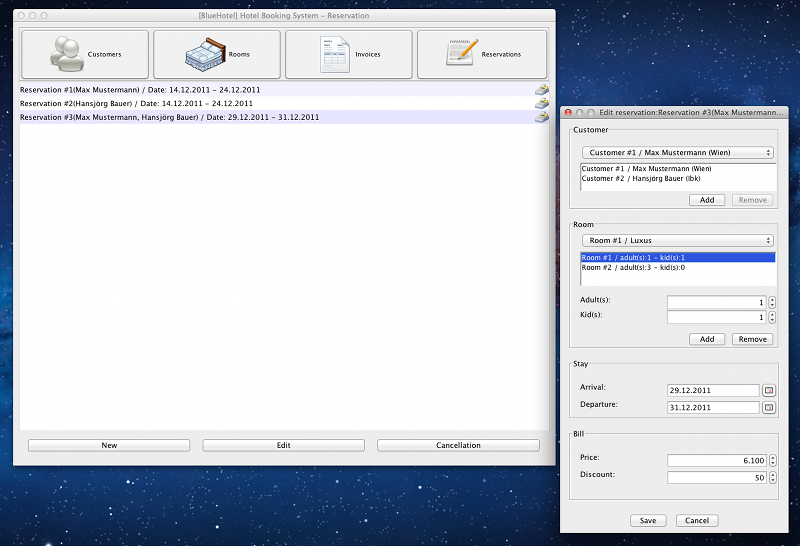
\includegraphics [width=0.7\textwidth] {img/demo.png}
\end{center}
\end{overprint}
\end{frame}

\section{}

\begin{frame}
\begin{center}
Danke f\"ur Ihre Aufmerksamkeit
\end{center}
\end{frame}

\end{document}